\documentclass{article}
\usepackage[letterpaper, margin=2cm]{geometry}
\usepackage{graphicx}
\title{\textbf{\huge{CSC343 Lab 2}}}
\date{}
\author{Yuchen Bao\\1004956880 \and Wen Hua Tung\\1004767040}


\begin{document}
\maketitle
\bigskip

\begin{enumerate}
    \item[1. ] \textbf{ER Diagram}\medskip\\
    \begin{figure}[htp]
    \centering
    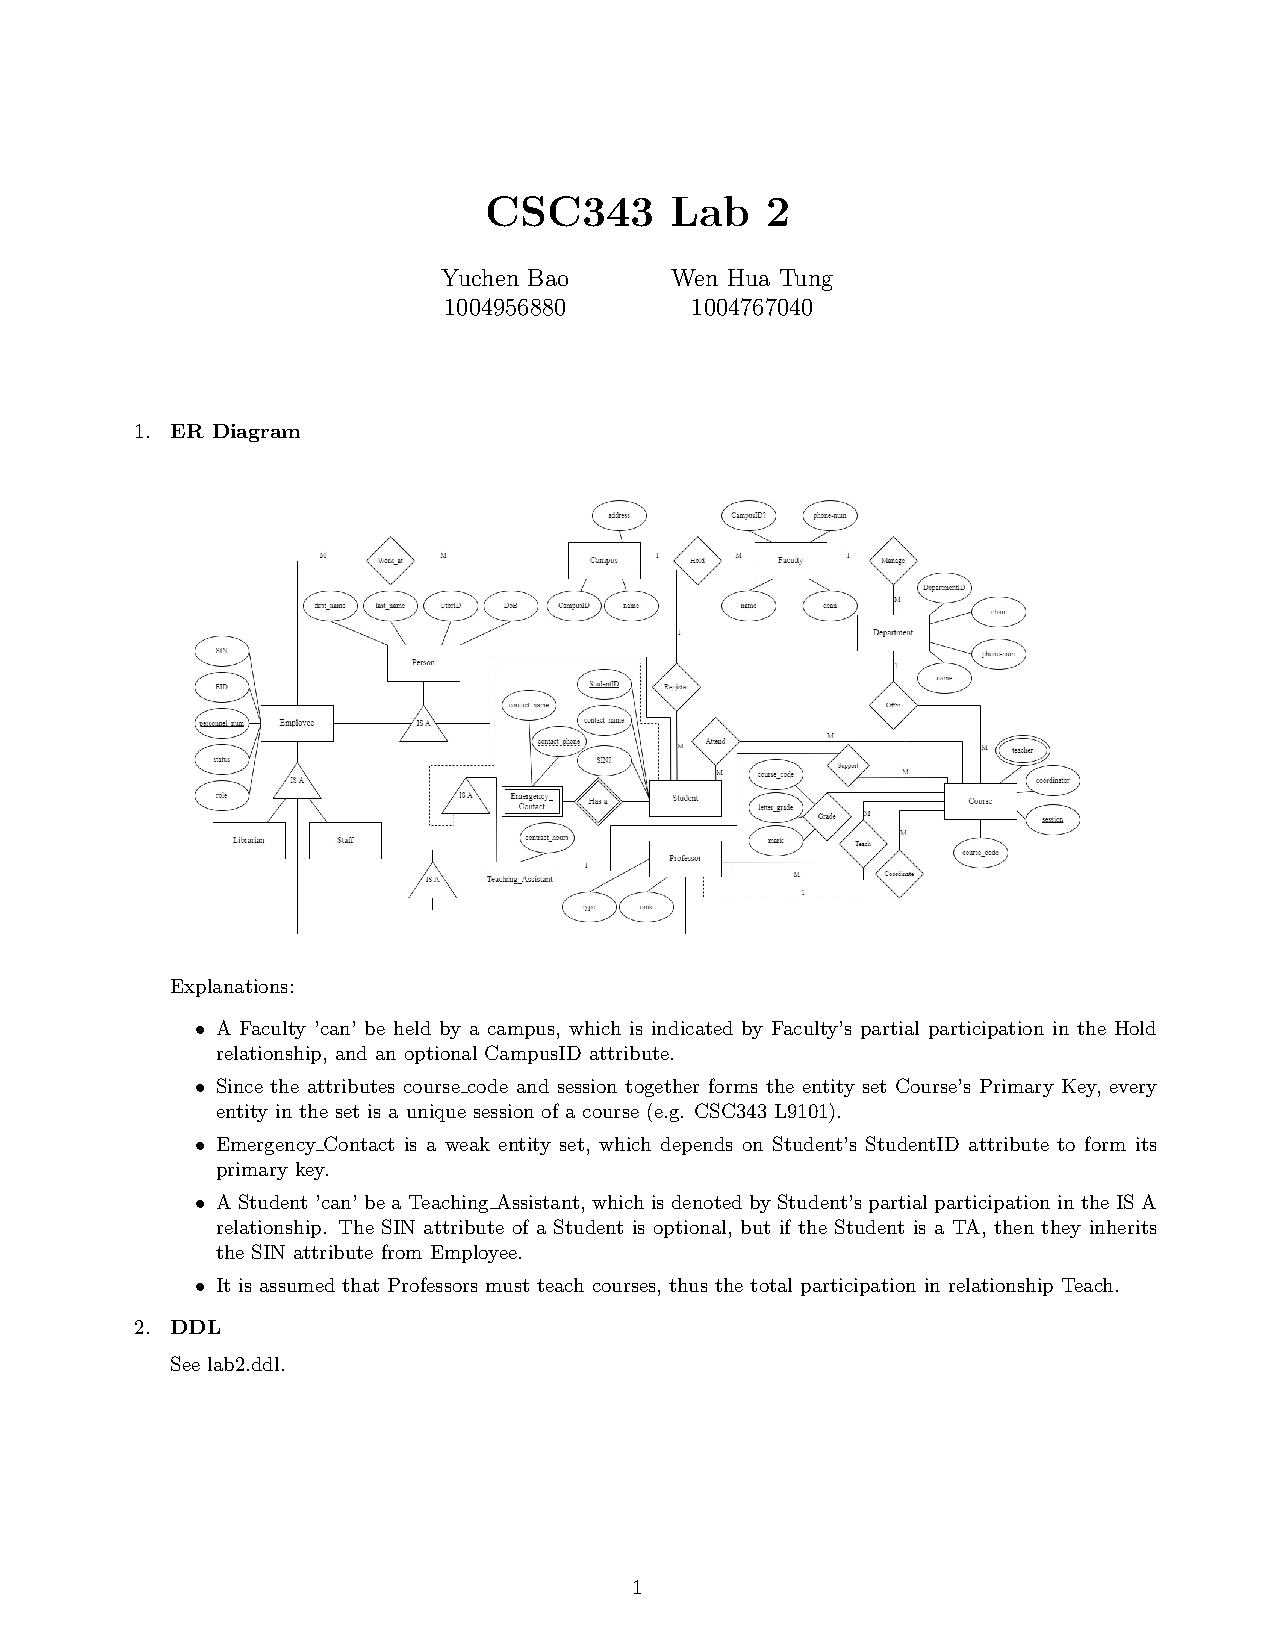
\includegraphics[width=15cm]{lab2.jpg}
    \end{figure}
    
    Explanations:
    \begin{itemize}
        \item A Faculty 'can' be held by a campus, which is indicated by Faculty's partial participation in the Hold relationship, and an optional CampusID attribute.
        \item Since the attributes course\_code and session together forms the entity set Course's Primary Key, every entity in the set is a unique session of a course (e.g. CSC343 L9101).
        \item Emergency\_Contact is a weak entity set, which depends on Student's StudentID attribute to form its primary key.
        \item A Student 'can' be a Teaching\_Assistant, which is denoted by Student's partial participation in the IS A relationship. The SIN attribute of a Student is optional, but if the Student is a TA, then they inherits the SIN attribute from Employee.
        \item It is assumed that Professors must teach courses, thus the total participation in relationship Teach.
    \end{itemize}
    
    \item[2. ] \textbf{DDL}\medskip\\
    See lab2.ddl.
\end{enumerate}

\end{document}
